\documentclass{article}
\usepackage{CJKutf8}
\usepackage{amsmath}
\usepackage{amsthm}
\usepackage{graphicx}
\begin{document}
\begin{CJK}{UTF8}{gbsn}
\newtheorem{Exercise}{习题}
\begin{Exercise}
  设$A$,$B$为有穷集合且$|A|=m, |B|=n$。

  a)计算$|A^B|=$?


  b)从$A$到$A$有多少个双射?
\end{Exercise}
\begin{proof}[解]
  $|A^B|=m^n$。

  从$A$到$A$有$m!$个双射。
\end{proof}
\begin{Exercise}
求证:从一个边长为$1$的等边三角形中任意选$5$个点,那么这$5$个点中必有$2$个点,它们之间的距离至多为$\frac{1}{2}$。而任选$10$个点中必有$2$个点,其距离至多为$\frac{1}{3}$。
\end{Exercise}

\begin{minipage}{0.49\linewidth}
  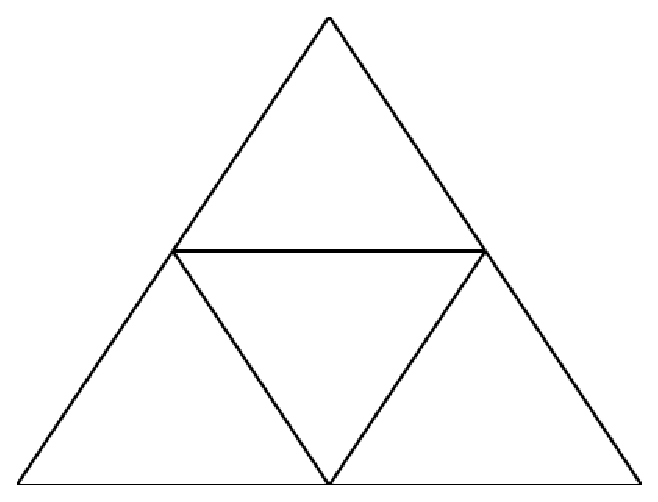
\includegraphics[width=4cm,height=3cm]{triangles2}
\end{minipage}
\begin{minipage}{0.49\linewidth}
  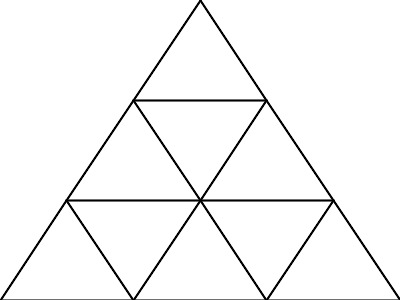
\includegraphics[width=4cm,height=3cm]{triangles3.jpg}
\end{minipage}

\begin{proof}[证明]




  (1)连接各边的中点,得到$4$个边长为$1/2$的小等边三角形。
  任给$5$个点,由鸽笼原理可知必有一个小等边三角形里面至少有两个点,又因为小等边三角形中任意两个点之间的距离至多为$1/2$,因此$5$个点中必有$2$个点,它们之间的距离至多为$1/2$。

(2)连接各边的三等分点,则可得到9个边长都为1/3的小等边小角形,每个小等边三角形中任意两个点之间的距离至多为1/3。将10个点放入该大等边三角形中,则由鸽笼原理,必有一个小等边三角形中至少有2个点,因此任意10个点中必有2个点其距离至多为1/3。
\end{proof}
\begin{Exercise}
  求证:在$52$个整数中,必有两个整数,使这两个整数之和或差能被$100$整除。
\end{Exercise}
\begin{proof}[证明]
  设$a_1,a_2,\cdots,a_{52}$为$52$个整数,令$r_i$为$a_i$被$100$除后所得的余数,即$a_i=100q_i+r_i,0\leq r_i \leq 99, i = 1,2,\cdots,52$(相当于$52$个物体)。

  任意一个整数被$100$除以后所得到的余数为$0,1,2,\cdots, 99$,把它们分成$51$个类,即$\{0\}, \{1,99\}, \{2,98\}, \cdots, \{49,51\}, \{50\}$(相当于$51$个盒子)。

  把$51$个余数$r_i$,$i=1,2,\ldots,52$,放入到$51$个类中,必有两个余数放在一个类里。

  设在同一个类中的两个余数分别为$r_i$与$r_j(i\neq j)$,则有

  (1)若$r_i\neq r_j$,则$r_i+r_j=100$或$0$,即$a_i+a_j$能被$100$整除。

  (2)若$r_i=r_j$,$r_i-r_j=0$,即$a_i-a_j$能被$100$整除。
\end{proof}
\begin{Exercise}
  设$f:X\to Y$,$C\subseteq Y$,$D\subseteq Y$,证明:$f^{-1}(C\setminus D)=f^{-1}(C)\setminus f^{-1}(D)$。
\end{Exercise}
\begin{proof}[证明]
  先证$f^{-1}(C\setminus D)\subseteq f^{-1}(C)\setminus f^{-1}(D)$。

  对任意的$x\in f^{-1}(C\setminus D)$,则$f(x)\in C\setminus D$,从而$f(x)\in C$并且$f(x)\notin D$,即$x\in f^{-1}(C)$并且$x\notin f^{-1}(D)$,因此$x\in f^{-1}(C)\setminus f^{-1}(D)$。

  再证$f^{-1}(C)\setminus f^{-1}(D)\subseteq f^{-1}(C\setminus D)$。

  对任意的$x\in f^{-1}(C)\setminus f^{-1}(D))$,则$x\in f^{-1}(C)$并且$x\notin f^{-1}(D)$,从而$f(x)\in C$并且$f(x)\notin D$,即$f(x)\in C\setminus D$,因此$x\in f^{-1}(C\setminus D)$。
\end{proof}
\begin{Exercise}
  设$f:X\to Y$,$A\subseteq X$,$B\subseteq X$。证明:$f(A\setminus B) \supseteq  f(A)\setminus f(B)$。
\end{Exercise}
\begin{proof}[证明]
对任意的$y\in  f(A)\setminus f(B)$,则$y\in f(A)$并且$y\notin f(B)$,从而存在$x\in A$使得$y=f(x)$。这里必有$x\notin B$,否则,$y=f(x)\in f(B)$,矛盾。因此,存在$x\in A\setminus B$使得$y=f(x)$,即$y\in f(A\setminus B)$。  
\end{proof}
\begin{Exercise}
  设$f:X\to Y$,$A\subseteq X$,$B\subseteq Y$。以下四个小题中,每个小题均有四个命题,这四个命题有且仅有一个正确。请找出正确的哪一个。

  (1)(a) 若$f(x)\in f(A)$,则$x$可能属于$A$,也可能不属于$A$;

  (b)若$f(x)\in f(A)$,则$x\in A$;

  (c)若$f(x)\in f(A)$,则$x\notin A$;

  (d)若$f(x)\in f(A)$,则$x\in A^c$。

  (2)(a) $f(f^{-1}(B))=B$;

  (b) $f(f^{-1}(B))\subseteq B$;

  (c) $f(f^{-1}(B))\supseteq B$;

  (d)$f(f^{-1}(B))= B^c$。

  (3)(a)$f^{-1}(f(A))=A$;

  (b) $f^{-1}(f(A))\subseteq A$;

  (c)$f^{-1}(f(A))\supseteq A$;

  (d)以上三个均不对。

  (4)(a)$f(A)\neq \phi$;

  (b)$f^{-1}(B) \neq \phi$;

  (c)若$y\in Y$,则$f^{-1}(\{y\})\in X$;

  (d)若$y\in Y$,则$f^{-1}(\{y\})\subseteq X$。
\end{Exercise}
\begin{proof}[解]
  (1)a (2)b (3)c (4)d
\end{proof}
\begin{Exercise}
  设$X=\{a,b,c\}$,$Y=\{0,1\}$,$Z=\{2,3\}$。$f:X\to Y$,$f(a)=f(b)=0$,$f(c)=1$;$g:Y\to Z$,$g(0)=2,g(1)=3$。试求$g\circ f$。
\end{Exercise}
\begin{proof}[解]
  $g\circ f:X\to Z, g\circ f(a)=2, g\circ f(b)=2, g\circ f(c)=3$。
\end{proof}
\begin{Exercise}
  设$N=\{1,2,\cdots\}$,试构造两个从集合$N$到集合$N$的映射$f$与$g$,使得$fg=I_N$,但$gf\neq I_N$。
\end{Exercise}
\begin{proof}[解]
  令$f:N\to N$,
  \[f(n)=
  \begin{cases}
    1& \text{当}n=1\text{时}\\
    n-1&\text{当}n>1\text{时}
  \end{cases}
  \]

  $g:N\to N$,对任意的$n\in N$,$g(n)=n+1$,则$fg=I_N$,但$gf\neq I_N$。
\end{proof}
\begin{Exercise}
设$f:X\to Y$。

(1)如果存在唯一的一个映射$g:Y\to X$,使得$gf=I_X$,那么$f$是否可逆呢?

(2)如果存在唯一的一个映射$g:Y\to X$,使得$fg=I_Y$,那么$f$是否可逆呢?
\end{Exercise}
\begin{proof}[解]

  (1)当$|X|=1$时,$f$不一定可逆,举例如下:

  设集合$X=\{1\}$,$Y=\{1,2\}$,$f:X\to Y$,$f(1)=1$。则存在唯一的一个映射$g:Y\to X$,$g(1)=1,g(2)=1$,使得$gf=I_X$,但$f$不可逆。

  当$|X|>1$时,$f$一定可逆,证明如下:

  由$gf=I_X$知$f$为单射,以下证明$f$为满射。用反证法,假设$f$不为满射,则存在$y_0\in Y$,对任意的$x\in X$,$f(x)\neq y_0$。
  由于$|X|>1$,可取$x_0\in X$,使得$g(y_0)\neq x_0$。

  令$h:Y\to X$,
  \[h(y)=\begin{cases}
      g(y) &\text{如果} y \neq y_0,\\
      x_0 &\text{如果} y = y_0\\
    \end{cases}
  \]
  则$hf=I_X$,且$h\neq g$,与存在唯一的一个映射$g:Y\to X$使得$gf=I_X$矛盾。
  

  (2)$f$一定可逆,证明如下:

  由$fg=I_Y$知$f$为满射,以下证明$f$为单射。用反证法,假设$f$不为单射,则存在$x_1\in X$,$x_2\in X$,$x_1\neq x_2$但$f(x_1)=f(x_2)$。

  设$y_0=f(x_1)=f(x_2)$,
  令$h:Y\to X$,
  \[h(y)=\begin{cases}
      g(y) &\text{如果} y \neq y_0,\\
      x_1 &\text{如果} y = y_0\text{且} g(y_0) \neq x_1\\
      x_2 &\text{如果} y= y_0 \text{且} g(y_0) = x_1
    \end{cases}
  \]
  则$fh=I_Y$,且$h\neq g$,与存在唯一的一个映射$g:Y\to X$使得$fg=I_Y$矛盾。
\end{proof}

\begin{Exercise}
设$f:X\to Y$,$X$与$Y$为有穷集合,

(1)如果$f$是左可逆的,那么$f$有多少个左逆映射?

(2)如果$f$是右可逆的,那么$f$有多少个右逆映射?
\end{Exercise}
\begin{proof}[解]
  (1) $|X|^{|Y|-|X|}$

(2) $\prod _{y\in Y}|f^{-1}(\{y\})|$
\end{proof}
\begin{Exercise}
是否有一个从$X$到$X$的一一对应$f$,使得$f=f^{-1}$,但$f\neq I_X$?
\end{Exercise}
\begin{proof}[解]
  存在。设集合$X=\{1,2\}$,$f:X\to X$,$f(1)=2$,$f(2)=1$,则$f=f^{-1}$,但$f\neq I_X$。
\end{proof}
\begin{Exercise}
 设$\sigma_1=\begin{pmatrix}1&2&3&4&5\\4&3&2&1&5\end{pmatrix}$,$\sigma_2=\begin{pmatrix}1&2&3&4&5\\3&2&5&1&4\end{pmatrix}$。求$\sigma_1\sigma_2$,$\sigma_2\sigma_1$,$\sigma_1^{-1}$,$\sigma_2^{-1}$。
\end{Exercise}
\begin{proof}[解]
  \begin{align*}
    &\sigma_1\sigma_2=\begin{pmatrix}1&2&3&4&5\\1&5&2&3&4\end{pmatrix}\\
    &\sigma_2\sigma_1=\begin{pmatrix}1&2&3&4&5\\2&3&5&4&1\end{pmatrix}\\
    &\sigma_1^{-1}=\begin{pmatrix}1&2&3&4&5\\4&3&2&1&5\end{pmatrix}\\
    &\sigma_2^{-1}=\begin{pmatrix}1&2&3&4&5\\4&2&1&5&3\end{pmatrix}\\
  \end{align*}
\end{proof}
\begin{Exercise}
  将置换$\sigma=\begin{pmatrix}1&2&3&4&5&6&7&8&9\\7&9&1&6&5&2&3&4&8\end{pmatrix}$分解成对换的乘积。
\end{Exercise}
\begin{proof}[解]
  \begin{align*}
    &\begin{pmatrix}1&2&3&4&5&6&7&8&9\\7&9&1&6&5&2&3&4&8\end{pmatrix}\\
    =&(173)(29846)\\
    =&(17)(13)(29)(28)(24)(26)\\
  \end{align*}
\end{proof}


\end{CJK}
\end{document}


%%% Local Variables:
%%% mode: latex
%%% TeX-master: t
%%% End:
